\documentclass[12pt,fleqn]{article}\usepackage{common}
\begin{document}
Spline Egrileri

Diyelim ki elimizde 4 $x_i,y_i$ noktasi var, ve bu noktalardan gecen (bu
onemli, tum noktalardan {\em kesinlikle} gecen) yaklasiksal bir egri
olusturmak istiyoruz. Spline yontemi her iki nokta arasini farkli bir
kupsel (ucuncu derece) polinom ile temsil etmektir. Tekrar dikkat: tum
noktalari temsile edebilecek farkli polinomlari toplamiyoruz, her aralikta
baska bir polinom fonksiyonunu devreye sokuyoruz. Peki parcalar niye
kupsel? Cunku kupsel bir egri yeterince kavis saglayabilir ve ayni zamanda
cok fazla inisli cikisli, sivri degildir.

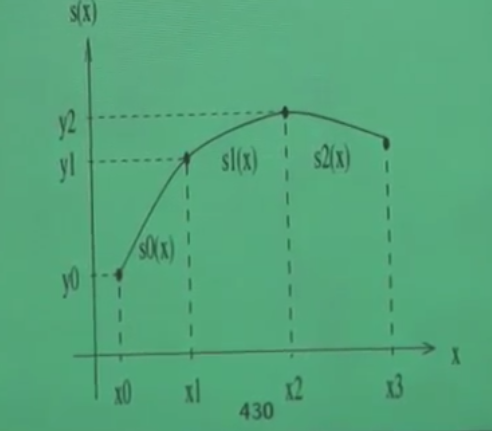
\includegraphics[height=4cm]{spline1.png}

Her $i=0,..,n-1$ icin 

\[ p(x) = p_i(x) = a_i + b_i(x-x_i) + c_i(x-x_i)^2 + d_i(x-x_i)^3
\ \ \ \label{1}
\]

kullanalim. Noktalar $x_i$ olarak gosteriliyor, ve her noktada aktif olan
bir $p_i$ spline olacak, o noktadan bir sonrakine kadar egriyi bu $s_i$
tanimlayacak. Peki her spline bir kubik polinom ise niye bu kubik polinomu
en basit sekliyle 

\[ p(x) = a_i + b_ix + c_ix^2 + d_ix^3 \]

olarak tanimlamadik? Cunku iki ustteki form ile calismak daha
rahat. Mesela, eger $x$ icin $x_i$ degrini verirsek, ki bu $x_1$ ya da
$x_2$ olabilirdi, o zaman parantez icinde $x_i - x_i$ sayesinde tum terimler sifir
oluyor, geriye sadece $a_i$ kaliyor. 

Parcalarin uclarinin birbirini tutmasi, ve tum seklin surekli, akiskan bir
sekilde gozukmesi icin ise birkac kosulu bizim tanimlamamiz, ve zorlamamiz
gerekli. Once en basit olani: bir onceki parca ile bir sonraki parca
orta nokta uzerinde ayni degere sahip olmali. $i=1,..,n+1$ icin

\[ p_i (x_{i+1}) = p_{i+1}(x_{i+1}) \]

Bir diger basit gereklilik, her $x_i$'ye tekabul eden spline fonksiyonun
elimizdeki $y_i$ degerini vermesi,

\[ p_i(x_i) = y_i \]

``Tum noktalardan kesinlikle gecmeli'' demistik. Son parca bir istisna
olusturuyor, o hem son nokta, hem de ondan bir onceki nokta icin gecerli
olmali

\[ p_{n-1}(x_n) = y_n \]

Genel yaklasim soyle, (1)'deki formulu ustteki gordugumuz her $p_i(x)$'in
yerine geciririz, bunu yapinca elimize bir lineer sistem gecer, $4n$ tane
denklem ve $4n$ tane bilinmez degiskenin oldugu bir denklem sistemi olur
bu, ve boyle bir sistemin cozumu vardir.

Sistemi daha detayli olarak gormek gerekirse..

Indisleri $i=1,..,n+1$ olarak tasarlayalim. Tum denklemleri yazarsak,

\[ p_1(x)  = a_1 + b_1(x-x_1) + c_1(x-x_1)^2 + d_1(x-x_1)^3\]

\[ p_2(x)  = a_2 + b_2(x-x_2) + c_2(x-x_2)^2 + d_1(x-x_2)^3\]

\[ \vdots \]

\[ p_3(x)  = a_3 + b_3(x-x_3) + c_3(x-x_2)^2 + d_3(x-x_2)^3\]

Uc noktali soyle bir grafik dusunelim,

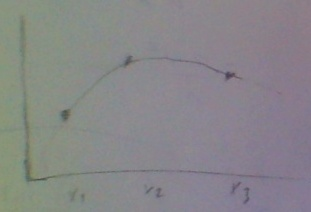
\includegraphics[height=4cm]{spline2.png}

Ustte bahsettigimiz gibi, $p_1(x_1) = a_1 = y_1$ olacak, ve tum indisler
icin bu gecerli. Ayrica $x_2$ noktasinda bir onceki parca ve sonraki parca
ayni degere sahip olmali demistik, yani mesela $p_1$'in sonunda (ustteki
ilk parca) $x_2$ noktasi vardir, ve ayni noktada $p_2$ baslayacaktir, o
noktada 

\[ p_1(x_2) = a_1 + b_1h_1 + c_1h_1^2 + d_1h_1^3  \]

ve bu denklem $p_2(x_2) = a_2 = y_2$'ye esit. Bir de, daha once gorduk, $a_1 =
y_1$ 
ise, o zaman 

\[ y_2 = p_1(x_2) = a_1 + b_1h_1 + c_1h_1^2 + d_1h_1^3 \]

haline gelir. Kisaca

\[ y_2 =  y_1 + b_1h_1 + c_1h_1^2 + d_1h_1^3 \]

Hepsini birarada yaziyoruz, tek basina olan $y$'yi sag tarafa aliyoruz

\[ y_1 + b_1h_1 + c_1h_1^2 + d_1h_1^3 = y_2 \]

\[ y_2 + b_2h_2 + c_2h_2^2 + d_2h_2^3 = y_3 \]

\[ \vdots \]

\[ y_n + b_nh_n + c_nh_n^2 + d_nh_n^3 = y_n \]

ki $h_1 \equiv x_2 - x_1$, $h_2 \equiv x_3 - x_2$ olarak tanimladik. Yani bir tur kisaltma 
olarak $h$ harfini kullaniyoruz. 

Fakat kesintisizlik icin parcalarin uclarinin bitismesi yeterli
degil. Mesela alttaki figur de uclari birlesik halde

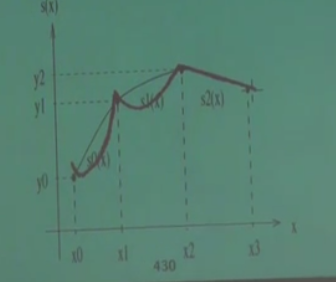
\includegraphics[height=4cm]{spline3.png}

Demek ki ek bazi sartlar lazim. Bu ek sart ``sureklilik'' olabilir. Mesela
alttaki ornek surekli degildir.

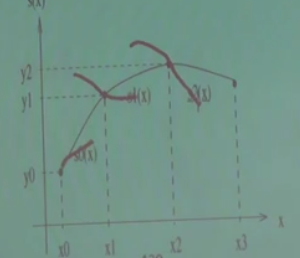
\includegraphics[height=4cm]{spline5.png}

Ya da daha iyisi, fonksiyonun her noktada ``turevi alinabilir'' olma
sarti. Mesela altta koyu yuvarlakli gosterilen noktada fonksiyonun turevi
alinamaz.

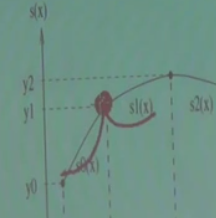
\includegraphics[height=4cm]{spline4.png}

O zaman sarti koyalim -- Fonksiyonun her noktasinda, ikinci turev surekli
alinabilmeli. Bu cok agir / net bir sart aslinda, ve hakikaten cok puruzsuz
(smooth) fonksiyonlara sebebiyet veriyor. Simdi bunun ne anlamina biraz
daha derinden bakalim. Bilirsiniz futbol sahalarinin etrafinda kosu alani
vardir. Bu alan soyledir.

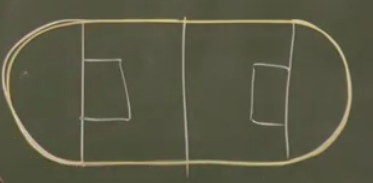
\includegraphics[height=4cm]{spline6.png}

Ustteki duz cizgili kisim sonsuz kere turevi alinabilir bir
fonksiyondur. Degil mi? Duz cizgi sabit bir sayidir, 1. turev sifir, ikinci
turev yine sifir, boyle gider. Peki yari cember olan kisimlar? Ayni
sekilde. Peki her noktada durum boyle midir? Kritik noktalar ufak yuvarlaklarla
gosterilen yerler (altta)

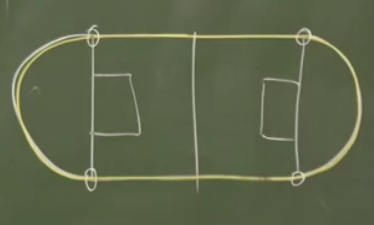
\includegraphics[height=4cm]{spline7.png}

Bu noktalarda kac kere ``surekli turevler'' alinabilir? Cevap, sadece bir
kere. Cunku iki kere turev alininca ne olacagina bakalim, duz kisimda
ikinci, ucuncu, vs. turev sifir. Peki yari cember? Onun ikinci turevi sifir
olmayan sabit bir sayi. o zaman tum fonksiyonun 2. turevini grafiklesek,
soyle bir grafik ortaya cikardi,

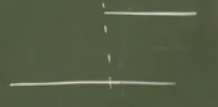
\includegraphics[height=2cm]{spline8.png}

ve bu grafikte goruyoruz ki bir ziplama var. Bu ziplama yuzunden sureklilik
(2. turevde) bozulmus oldu.

O zaman spline duzgun, puruzsuz olsun istiyorsak, her noktada, yani
baglanti noktalarinda, sagdaki ve soldaki parcanin birinci ve ikinci
turevinin ayni olmasi sartini koyabiliriz, o zaman bu noktalarda
fonksiyonun tamami iki kere surekli turevi alinabilir hale
gelir. Parcalarin kendisi uzerinde bu sarti tanimlamaya gerek yok, cunku
orada polinom kullanacagimizi belirttik zaten, polinomlar sonsuz kere
surekli turevi alinabilen objelerdir. 

Denklem sistemimize iki tane daha sart gerekiyor. Bu sartlar fonksiyonun
ilk noktada ve son noktada ikinci turevinin sifir olmasi sarti
olabilir. Her hangi yondeki bir cizgi $y = ax + b$'nin iki kere turevi
alininca sifir gelir, yani bu sart fonksiyonumuzun son noktalarda,
fonksiyonun ``asagi yukari ayni yonde'' olacak sekilde duz olarak devam
etmesi anlamina geliyor. Yaklasiksal baglamda fena bir sart degil. 

O zaman ana formullerimize donelim, ve mesela $p_1(x),p_2(x)$'in turevini
alalim,

\[ p_1'(x) = b_1 + 2c_1h_1 + 3d_1h_1^2 \]

\[ p_2'(x) = b_2 + 2c_2h_2 + 3d_2h_2^2 \]

\[ \vdots \]


Turevleri esitleyelim $p_1'(x_2) = p_2'(x_2)$. 

\[ p_1'(x_2) = b_1 + 2c_1h_1 + 3d_1h_1^2 \]

\[  p_2'(x_2) = b_2 \]

Ustteki niye sadece $b_2$ oldu? Cunku $x_i-x_i$ numarasi onun icin de
gecerli, geriye sadece $b_2$ kaldi. Hepsi bir arada

\[  b_1 + 2c_1h_1 + 3d_1h_1^2  = b_2 \]

\[  b_2 + 2c_2h_2 + 3d_2h_2^2 = b_3 \]

\[ \vdots \]

\[  b_{n-1} + 2c_{n-1}h_{n-1} + 3d_{n-1}h_{n-1}^2 =  b_n \]

Ikinci turevler icin benzer bir durum var, bu sefer sol taraftan $b$'ler
yokoluyor, 

\[ 2c_1 + 6d_1h_1 = 2c_2 \ \ \ \label{2} \]

\[ 2c_2 + 6d_2h_2 = 2c_3 \]

\[ \vdots \]

\[ 2c_{n-1} + 6d_{n-1}h_{n-1} = 2c_n \]

Ilk ve son ikinci turevi sifira esitlemeyi unutmayalim. Son turev

\[ 2c_n + 6d_nh_n = 2c_{n+1} = 0 \]

Ilk turev
\[ p_1''(x_1) =  c_1 + \cancelto{0}{6d_1(x_1-x_1)}  = c_1 = 0\]

Denklem (2)'den baslayan blogu tekrar duzenlersek, 
















http://spartan.ac.brocku.ca/~jvrbik/MATH2P20/notes.pdf

http://www.youtube.com/watch?v=3rHBCglD1LQ

http://www.youtube.com/watch?v=nA0YpqraP9A


\end{document}
